%======================================================================
\section{The experiments and what they show}
%======================================================================

\subsection{The central difficulty: there is no ``true symmetry'' label}
No public dataset says ``this face is 2.3\% asymmetric''. So we built two kinds of test.
\begin{enumerate}
\item \textbf{Reference from expert landmarks ($A_{ref}$).} We apply \emph{exactly the same}
measurement to the 68 points placed by human experts. If our detector-based measurement
agrees with $A_{ref}$, our pipeline measures what an expert-landmark measurement would.
$A_{ref}$ is not perfect truth (experts make small errors too), but it is the best reference
available.
\item \textbf{Controlled perturbations.} We degrade each test photo in known ways
(brightness, blur, covering a part, rotation, shrinking). The face itself does not change, so
the correct answer does not change either. Any change in the score is an error.
\end{enumerate}

\textbf{Two metrics we defined (know these well):}
\begin{itemize}
\item \textbf{Silent failure}: the system \emph{reports} a score (does not reject), but it is
off from $A_{ref}$ by more than 1\% IOD. This threshold was fixed before running and is about
twice the normal error. This is the failure a gate exists to prevent.
\item \textbf{Drift}: the median change of the score between the clean and the degraded photo,
divided by how much scores normally vary between people (the SD of clean scores). Dividing
by the SD lets us compare the baseline (face-width units) with ours (IOD units).
\end{itemize}

\subsection{E1--E3: do we agree with the experts?}
\begin{center}\begin{tabular}{@{}lccc@{}}
\toprule
Measure ($n$=224) & $\rho$ & $r$ & MAE\\
\midrule
M0 baseline~\cite{nashokan_facialasymmetry} (KD-tree, vert.\ midline) & 0.823 & 0.762 & --\\
\quad M0 w/o alignment & 0.614 & 0.630 & --\\
\quad M0 + fixed pairs (no KD-tree) & 0.931 & 0.903 & --\\
M1: 68-pt pairs + fitted axis & 0.938 & 0.951 & 0.45\\
M3: M1 + mirror averaging & 0.947 & 0.957 & 0.45\\
\bottomrule
\end{tabular}
\end{center}
\begin{figure}[h]\centering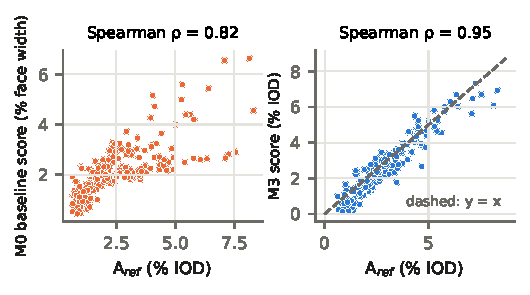
\includegraphics[width=0.7\linewidth]{agreement.pdf}
\caption{Each dot is one test face. Left: baseline. Right: ours, close to the $y=x$ line.}\end{figure}
\textbf{How to read it:} replacing \emph{only} the KD-tree matching with fixed pairs (same
detections, same midline) already raises $\rho$ from \rhoMzero{} to \rhoMzeroFixed{}. So
\emph{wrong correspondence was the baseline's main problem}. The fitted axis on the 68-point
layout gives \rhoMone{} (average error \maeMone\% IOD), and mirror averaging gives \rhoMthree{}.

\textbf{Regions and shrinkage (E3).} Regional agreement is 0.84--0.98. The detector's
asymmetry is systematically \emph{smaller} than the experts': by \shrinkGlobal\% overall and
\shrinkMouth\% at the mouth (statistically significant everywhere except the brows).
MediaPipe has a built-in ``average face'' prior that pulls unusual (asymmetric) shapes
towards symmetry. So our regional numbers should be read as conservative.

\subsection{E8: head pose dominates in-the-wild asymmetry}
\begin{figure}[h]\centering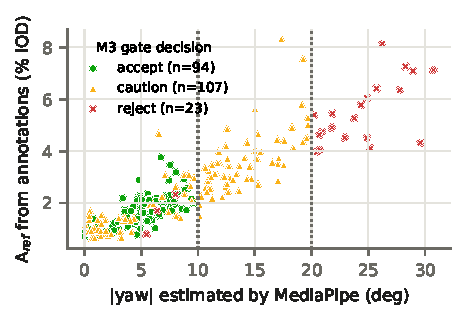
\includegraphics[width=0.55\linewidth]{pose_confound.pdf}
\caption{Asymmetry from expert landmarks against head yaw. Dotted lines: gate limits.}\end{figure}
\begin{center}\begin{tabular}{@{}lccccc@{}}
\toprule
$|$yaw$|$ (deg) & n & A$_{ref}$ & M1 & $|$err$|$ M3 & NME\\
\midrule
0-5 & 77 & 1.20 & 0.80 & 0.47 & 3.03\\
5-10 & 67 & 2.14 & 1.86 & 0.40 & 5.51\\
10-20 & 60 & 3.60 & 3.41 & 0.42 & 3.32\\
$\geq$20 & 20 & 5.50 & 5.42 & 0.57 & 4.13\\
\bottomrule
\end{tabular}
\end{center}
\textbf{How to read it:} even from expert landmarks, asymmetry rises from \yawLow\% to
\yawHigh\% as yaw grows ($\rho$ = \rhoYawRef{}). This is a property of 2D photos, not of
our detector. The detector's error (``$|$err$|$ M3'') stays about the same at every yaw. That
is exactly why a separate pose check is needed: a check that only looks at detector error
would not catch it. Among gate-accepted faces the correlation falls to \rhoYawRefAcc{}.

\begin{careful}
The pose groups contain \emph{different people} (each LFPW person appears once). Do not say
``the same face measured at different angles''.
\end{careful}

\subsection{Does the mirror test find bad landmarks?}
\begin{figure}[h]\centering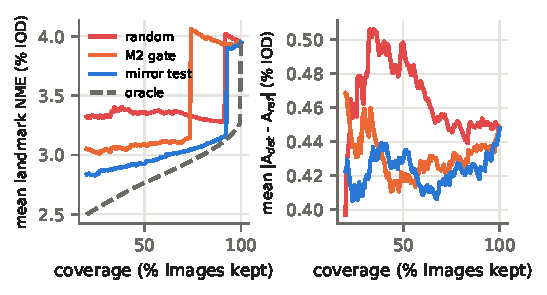
\includegraphics[width=0.62\linewidth]{risk_coverage.pdf}
\caption{Risk--coverage. Keep the images the signal trusts most; the y-axis is the average error
of the kept images (lower is better).}\end{figure}
\textbf{Risk--coverage curve:} sort images from most to least trusted by a signal and keep the
top $x$\%. A good signal keeps low-error images first. The area under the curve (AURC)
summarises it: lower is better.
\begin{itemize}
\item For landmark error (left): random \aurcRandom{}, gate signals without the mirror test
\aurcGateTwo{}, \textbf{mirror test \aurcMirror{}}, perfect oracle \aurcOracle{}. The mirror
test closes \gapClosed\% of the gap between random and perfect.
\item For the asymmetry error on clean photos (right), no signal does much better than random
(\aurcAsymMirror{} vs.\ \aurcAsymRandom{}). On clean photos, most landmark errors are similar on
both sides and cancel in $A$. The gate pays off on degraded photos (next section).
\end{itemize}

\subsection{E4--E7: robustness to degraded photos}
26 settings $\times$ 224 faces = 5{,}824 degraded images: brightness $\times$0.25 to $\times$2.5,
blur of 1--8\% of IOD, a grey box over one eye/nose/mouth, rotation $\pm$5--30$^\circ$, and
shrinking to 50--12\% of the size.
\begin{figure}[h]\centering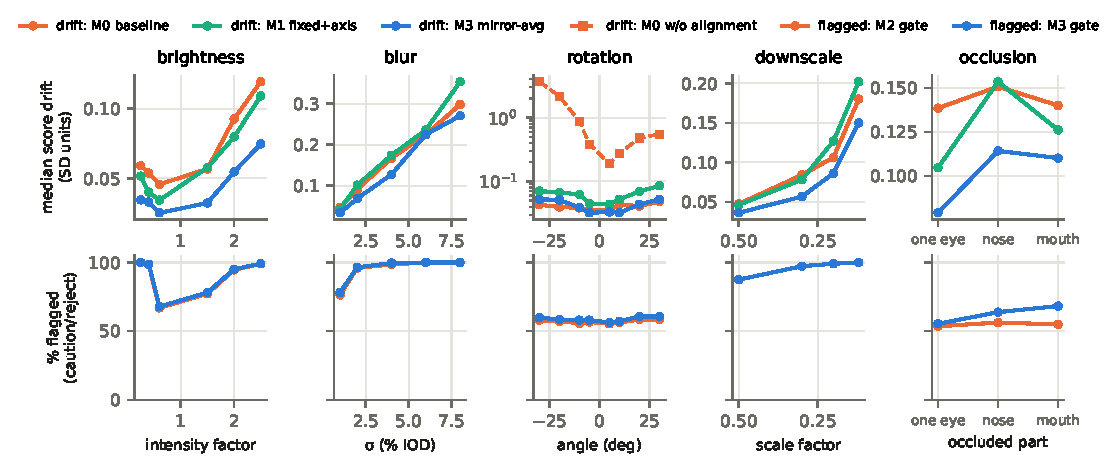
\includegraphics[width=\linewidth]{robustness.pdf}
\caption{Top: drift (lower is better). Bottom: \% of images the gate flags.}\end{figure}
\textbf{How to read it:}
\begin{itemize}
\item MediaPipe still finds a face in at least \detMin\% of images in every setting. So the
risk is not ``no answer'' but a \emph{plausible-looking wrong answer}.
\item Blue (mirror averaging) drifts least under every type of degradation.
\item Rotation panel (log scale): the vertical-midline method without alignment drifts by up to
\rotNoAlignMax{} SD. Our fitted axis stays below \rotMthreeMax{} SD with no re-detection.
\item The gate flags more and more images as blur, darkness or shrinking increase, which is what
we want.
\end{itemize}

\subsection{E9: ablation (what each component contributes)}
\begin{center}\small\begin{tabular}{@{}llcccccc@{}}
\toprule
Setting & Var. & n & Reported & Accepted & $\rho$ & Silent fail. & Drift\\
 & & & (\%) & (\%) & vs ref & (\%) $\downarrow$ & (SD) $\downarrow$\\
\midrule
Clean test & M0 & 224 & 100.0 & 100.0 & 0.823 & -- & --\\
 & M1 &  & 100.0 & 100.0 & 0.938 & 5.8 & --\\
 & M2 &  & 90.2 & 43.3 & 0.921 & 4.9 & --\\
 & M3 &  & 89.7 & 42.0 & 0.932 & 4.0 & --\\
\midrule
Perturbed, pooled & M0 & 5824 & 98.4 & 98.4 & 0.814 & -- & 0.070\\
 & M1 &  & 98.4 & 98.4 & 0.921 & 8.1 & 0.076\\
 & M2 &  & 64.0 & 22.6 & 0.918 & 3.4 & =\\
 & M3 &  & 63.2 & 21.0 & 0.927 & 3.6 & 0.054\\
\midrule
\quad blur & M0 & 1120 & 94.0 & 94.0 & 0.787 & -- & 0.131\\
 & M1 &  & 94.0 & 94.0 & 0.870 & 14.4 & 0.130\\
 & M2 &  & 37.0 & 5.8 & 0.903 & 2.7 & =\\
 & M3 &  & 35.6 & 5.2 & 0.919 & 2.3 & 0.099\\
\midrule
\quad downscale & M0 & 896 & 98.7 & 98.7 & 0.821 & -- & 0.087\\
 & M1 &  & 98.7 & 98.7 & 0.909 & 9.2 & 0.097\\
 & M2 &  & 33.5 & 4.0 & 0.919 & 1.8 & =\\
 & M3 &  & 33.4 & 4.0 & 0.927 & 1.9 & 0.066\\
\midrule
\quad brightness & M0 & 1344 & 99.5 & 99.5 & 0.818 & -- & 0.065\\
 & M1 &  & 99.5 & 99.5 & 0.936 & 5.8 & 0.056\\
 & M2 &  & 62.8 & 10.6 & 0.927 & 2.8 & =\\
 & M3 &  & 62.4 & 10.2 & 0.940 & 2.7 & 0.037\\
\midrule
\quad occlusion & M0 & 672 & 98.8 & 98.8 & 0.804 & -- & 0.142\\
 & M1 &  & 98.8 & 98.8 & 0.919 & 8.8 & 0.124\\
 & M2 &  & 87.9 & 45.1 & 0.900 & 6.2 & =\\
 & M3 &  & 85.1 & 37.5 & 0.911 & 6.0 & 0.098\\
\midrule
\quad rotation & M0 & 1792 & 100.0 & 100.0 & 0.825 & -- & 0.039\\
 & M1 &  & 100.0 & 100.0 & 0.944 & 5.2 & 0.059\\
 & M2 &  & 88.1 & 43.0 & 0.924 & 4.0 & =\\
 & M3 &  & 87.7 & 41.4 & 0.928 & 4.9 & 0.040\\
\bottomrule
\end{tabular}
\end{center}
\textbf{How to read it:} without a gate (M1), \silentPoolOne\% of degraded measurements are
silent failures (\silentBlurOne\% under blur). With the gate (M2/M3) this falls to
\silentPoolTwo\%/\silentPoolThree\% (\silentBlurThree\% under blur). The price is coverage:
only \covPoolThree\% of degraded and \covCleanThree\% of clean images still get a score. M3 has
the lowest drift (\driftPoolThree{} vs.\ \driftPoolOne{} SD).

\subsection{Gate behaviour on clean photos, and an honest negative result}
On the clean test set M3 accepts \pAccept\%, cautions \pCaution\% and rejects \pReject\%
of faces. Pose is the main trigger: LFPW faces are mostly turned. Accepted faces have a lower
landmark error (\nmeAccept\% vs.\ \nmeCaution\% NME).

\textbf{Negative result:} when a grey box covers the nose or mouth, the region is flagged
unreliable in \occNose\% and \occMouth\% of faces. When it covers an \emph{eye}, it is
flagged in only \occEye\%. MediaPipe ``invents'' the hidden eye from its average-face prior,
the same way in both the photo and its mirror, so the mirror test sees agreement. Lesson:
\emph{the mirror test catches inconsistent landmarks, not confidently invented ones.} An
appearance-based occlusion check is future work.

%======================================================================
\section{The code, file by file}
%======================================================================
\begin{center}\small
\begin{tabular}{@{}p{4.4cm}>{\raggedright\arraybackslash}p{11cm}@{}}
\toprule
File & What it does\\
\midrule
\texttt{src/fsm/detector.py} & Loads MediaPipe once; \texttt{detect(img)} returns 478 points, the pose matrix and the number of faces; \texttt{pose\_from\_transform} turns the matrix into yaw/pitch/roll.\\
\texttt{src/fsm/mesh.py} & Mirror permutation from the canonical model; the 68-point pairs and regions; the fitted 478$\to$68 map.\\
\texttt{src/fsm/geometry.py} & All the maths: reflection, fitted axis, asymmetry $a_i$, $A$, $A_r$; the baseline KD-tree method; un-flipping and mirror inconsistency.\\
\texttt{src/fsm/quality.py} & Sharpness/brightness/clipping on the face crop; \texttt{gate\_decision} (accept/caution/reject + reasons); \texttt{risk\_score}.\\
\texttt{src/fsm/pipeline.py} & \texttt{raw\_detect} (all detector calls) and \texttt{measure\_from\_raw} (all geometry); \texttt{variant\_outputs} turns one measurement into M0--M3.\\
\texttt{src/fsm/viz.py} & Drawing: mesh, axis, pairs, residuals, heatmap, status banner.\\
\texttt{src/fsm/data.py} & Reads LFPW \texttt{.pts} files; crops to the annotated face.\\
\texttt{app.py} & Streamlit interface; it only \emph{calls} the engine, with no maths in the UI.\\
\texttt{experiments/} & Run in order: \texttt{cache\_detections} $\to$ \texttt{fit\_mp68\_mapping} $\to$ \texttt{calibrate\_gate} $\to$ \texttt{run\_clean\_eval} $\to$ \texttt{run\_perturbations} $\to$ \texttt{summarize\_perturbations} $\to$ \texttt{make\_figures}, \texttt{make\_tables}.\\
\texttt{configs/} & Canonical face model, fitted map, gate limits (JSON); no thresholds are hard-coded in the UI.\\
\texttt{tests/test\_geometry.py} & 15 unit tests: reflection, zero score for a symmetric face, rotation/scale invariance, known displacement, un-flip round trip, mirror-consistent map, gate levels.\\
\bottomrule
\end{tabular}
\end{center}
\textbf{Design choices you may be asked about:} the engine never imports Streamlit, so the
same code runs the app and the experiments. Detections are cached once, so every variant
is scored on identical landmarks. Every table and figure in the paper is written by a
script from saved CSVs, so no number was typed by hand.

%======================================================================
\section{The app, screen by screen}
%======================================================================
\begin{itemize}
\item \textbf{Sidebar}: choose upload or webcam; ``stress-test'' sliders (brightness, blur,
rotation, occlusion) to show the gate reacting live; a toggle to show the baseline's number.
\item \textbf{Verdict}: green/amber/red box with the reasons (for example ``head is turned
left/right''). For reject the score shows ``withheld''.
\item \textbf{Numbers}: asymmetry $A$ (\% IOD), mirror stability $\pm$, symmetry index (0--100).
\item \textbf{Overlays tab}: mesh; fitted axis with pairs; green point vs.\ red reflection of
its twin; heatmap (grey = unreliable region).
\item \textbf{Regions tab}: table and bar chart for the five regions, with reliable/unreliable status.
\item \textbf{Quality signals tab}: each signal's value next to its caution/reject limits, and the pose angles.
\item \textbf{Export tab}: JSON and CSV download.
\end{itemize}

%======================================================================
\section{How to present it}
%======================================================================
\textbf{The story in four sentences:}
(1) Symmetry tools give a number for every photo, but 2D photos are easily dominated by
pose and image quality. (2) We measure with correct anatomical pairs and a fitted axis, check
the landmarks with a mirror test, and gate on quality and pose. (3) Against expert landmarks and
under 26 degradations, this agrees much better and prevents most silent failures. (4) We are
honest about what it cannot do: occluded eyes, shrinkage, 2D pose.

\textbf{Suggested split} (change to match who actually did what):
slides 1--5 Pankaj; 6--9 Prutha and Ashish; 10--14 Ankit and Ashish; 15 Pankaj;
16 (demo) Mahi; 17 Prutha. The speaker notes on every slide hold the details, and
\texttt{presentation/DEMO\_SCRIPT.md} has the step-by-step demo.

\textbf{Timing for about 12 minutes:} problem and motivation 2 min; related work and
contributions 1.5 min; method 3 min; results 3 min; failures 1 min; demo 2--3 min.

%======================================================================
\section{Questions you should be ready for}
%======================================================================
\begin{description}[style=nextline,leftmargin=0pt,itemsep=5pt]
\item[What exactly is novel?] Not landmarks, regions or the UI; those exist. Our novelty is
(1) fixed anatomical pairs plus a fitted axis, which fixes the \kdWrong\% wrong-partner
problem and raises agreement from \rhoMzero{} to \rhoMthree{}; (2) the mirror test as a
label-free reliability signal and bias-cancelling average; (3) a train-calibrated gate
evaluated by silent failures and coverage; (4) the evaluation protocol.
\item[How do you know your score is right without labels?] We compare with the identical
measure on expert landmarks, and we use degradations where the answer is known not to
change. We do not claim agreement with human symmetry \emph{ratings}; we have none.
\item[Why not just align the face like the baseline?] Alignment needs a second detection
and still relies on two points being correct. The fitted axis is mathematically
rotation-invariant and uses all 51 inner points.
\item[Why IOD and not face width?] IOD is the 300-W standard and does not depend on the jaw
outline, which moves with pose.
\item[Did you tune thresholds on the test set?] No. Pose and size limits were set a priori;
the rest are training-set percentiles. The test set was only evaluated.
\item[Why does the gate reject so many LFPW faces?] LFPW is in-the-wild: about two thirds of
test faces are turned more than 5$^\circ$. Given $\rho$ = \rhoYawRef{} between yaw and
asymmetry, refusing those is correct behaviour.
\item[Why not train a deep network?] There are no symmetry labels to train on, and explicit
geometry is interpretable and unit-testable. Training a detector was out of scope.
\item[Could MediaPipe have seen LFPW in training?] Possibly; its training data is not public.
That is why we do not present its NME as an independent benchmark result, only as a
comparison between our mappings and signals.
\item[What is the 0--100 index?] A monotone re-expression of $A$ for readability, with the
median training face at 50. It is not a validated scale.
\item[Is this a medical or attractiveness score?] No. It is a 2D geometric indicator, and the
app says so.
\item[Did you copy code?] No. The audited repositories have no licence, so we
re-implemented the baseline method ourselves. The MediaPipe model and canonical mesh are
Apache-2.0.
\item[What would you do next?] Use MediaPipe's 3D landmarks to undo yaw and validate on
AFLW2000-3D (which has true pose); add an appearance-based occlusion check; use WFLW subsets;
collect consented multi-pose photos with human symmetry ratings.
\end{description}

%======================================================================
\section{Glossary}
%======================================================================
\begin{description}[leftmargin=0pt,itemsep=1pt]
\item[$A$ / $A_r$] global / regional asymmetry, in \% IOD.
\item[$A_{ref}$] the same measure computed from expert landmarks (the reference).
\item[AURC] area under the risk--coverage curve; lower is better.
\item[Bilateral pair] a point and its mirror twin on the other side of the face.
\item[Canonical face model] MediaPipe's exactly symmetric 3D average face.
\item[Caution / reject] the gate's warning level / refusal level.
\item[$\delta$, $\delta_r$] mirror inconsistency (whole inner face / one region), as a fraction of IOD.
\item[Drift] median score change under degradation, in units of the between-person SD.
\item[IOD] inter-ocular distance (outer eye corner to outer eye corner).
\item[KD-tree] a data structure for fast nearest-neighbour search; the baseline uses it to match points.
\item[LFPW / 300-W] the benchmark with 68 expert landmarks per face that we used.
\item[M0--M3] baseline, fixed pairs + axis, + gate, full system.
\item[NME] landmark error divided by IOD.
\item[$\pi$] the mirror permutation: $\pi(i)$ is the twin of point $i$.
\item[Silent failure] a reported score that is off by more than 1\% IOD.
\item[Yaw / pitch / roll] turning left--right / nodding / tilting to a shoulder.
\end{description}
